% mod1_main.tex

\documentclass[10pt,letterpaper]{article}

\title{Module 1}

\usepackage{fullpage}
\usepackage{graphicx}
\usepackage{framed}
\usepackage[labelfont=bf]{caption}
\usepackage{subcaption}
\usepackage{nopageno}
\pagestyle{plain}
\usepackage{array}
\usepackage[export]{adjustbox}
\usepackage{tabularx} % table features
\usepackage{booktabs} % table features
\usepackage[abs]{overpic} % overlaying one graphic on another
\usepackage{xstring,xifthen} % string length with conditionals
\usepackage{color} % colored text
\usepackage{xcolor}
\usepackage{helvet} % font
\usepackage{lipsum}

% Font colors
\definecolor{agpBrown}{rgb}{0.3490196,0.2352941,0.2196078}
\definecolor{agpRust}{rgb}{0.6627451,0.2196078,0.1411765}
\definecolor{agpMustard}{rgb}{0.8666667,0.7254902,0.1490196}
\definecolor{agpFlesh}{rgb}{0.9607843,0.8431373,0.7725490}
\definecolor{agpBlue}{rgb}{0.1294118,0.1882353,0.3960784}
\definecolor{agpRed}{rgb}{0.7490196,0.1254902,0.2000000}
\definecolor{agpGray}{rgb}{0.9333333,0.9254902,0.9254902}

% Font sizes Helvetica
\def\twelvept{\fontfamily{phv}\fontsize{12}{14}\selectfont}
\def\tenpt{\fontfamily{phv}\fontsize{10}{12}\selectfont}
\def\eightpt{\fontfamily{phv}\fontsize{8}{10}\selectfont}

% Margins
\topmargin -1.5cm
\oddsidemargin -1.5cm
\textwidth 19.5cm 
\textheight 27.6cm
\footskip 1.0cm
\parindent=0pt
\baselineskip=0pt
\parskip=10pt

% My itemize environment
\newenvironment{my_itemize}{
\begin{itemize}
  \setlength{\itemsep}{1pt}
  \setlength{\parskip}{0pt}
  \setlength{\parsep}{0pt}}{\end{itemize}
}

% Top align table cell
\def\topalign#1{\vtop{\null\hbox{#1}}}

% Colorbox spacing
{\setlength{\fboxsep}{0pt}

% Line spacing
\linespread{1.1}

% Load helvetica for sans serif
\renewcommand\sfdefault{phv}

% Use sans serf font throughout
\renewcommand{\familydefault}{\sfdefault}

% Macros
%\input{mod1_macros_static.tex}
%\input{mod1_macros_dynamic.tex}
% mod1_macros.tex


% release date
\def\releaseDate{June 11, 2014}


% participants paragraph

\def\numSamples{3,831}

\def\numParticipants{3,238}
\def\pgpParticipants{86}


% participants table
\def\hmpAge{Adults}
\def\hmpLocation{USA}
\def\hmpSamples{4,788}
\def\hmpParticipants{242}
\def\hmpSequences{36,797,226}
\def\ggAge{Adults,Children}
\def\ggLocation{Venezuela, Malawi, USA}
\def\ggSamples{531}
\def\ggParticipants{531}
\def\ggSequences{1,093,740,274}
\def\pgpAge{Adults}
\def\pgpLocation{USA}
\def\pgpSamples{439}
\def\pgpParticipants{86}
\def\pgpSequences{9,509,776}
\def\agpAge{Adults, Children}
\def\agpLocation{Global}
\def\agpSamples{3,831}
\def\agpParticipants{3,238}
\def\agpSequences{101,435,579}


% diversity figure
\def\numParticipantsLowerEstimate{3,238}


%%%%%%%%%% BEGIN DOCUMENT %%%%%%%%%%

\begin{document}

% PAGE 1
\parbox{4.5cm}{
	
\includegraphics[width=0.2\textwidth]{pdfs-mod1/logoshape.pdf}
}
\parbox{14cm}{
	\fontsize{20pt}{24pt}\selectfont
	Preliminary Characterization of \\ the American Gut Population
}

\vspace{0.5cm}

As of \releaseDate{}, we have completed sequencing and analysis of gut, skin, and oral bacteria from the first \numSamples{} samples of \numParticipants{} participants in the American Gut study.  This document gives us a summary of the most up-to-date results for the whole population. 

Here we compare the American Gut population to other populations who have had their gut, oral, and skin bacteria characterized.  We then describe the participants in the study, show the major kinds of bacteria in the gut microbiota of the American Gut population, and provide some information about what affects gut bacteria (as well as show that some variables such as gender have surprisingly little effect).

{\em Technical note: ``microbiota'' refers to a particular community of microbes, including bacteria (e.g., the human gut microbiota); ``microbiome'' refers to the genes those microbes contain (e.g., the human gut microbiome). Most participants in American Gut have signed up for characterization of the microbiota.}

% HEADING 1.1
\colorbox{agpFlesh}{\parbox{\textwidth}{\vspace{1mm} \LARGE \centering A map of your microbes \vspace{1mm}}}

A useful way to compare thousands of microbiota samples at the same time is by putting them on a map where more similar samples are closer together, and more dissimilar ones are further apart.

{\bf Figure 1A} shows how the microbes from different parts of the body relate to one another: as you can see, the fecal (gut), oral and skin microbiota form three points of a triangle, reflecting the major differences between these body locations. (Amazingly, even the same person has essentially none of the same bacteria in their skin, their mouth, and their gut.) In these figures, we compare the data from American Gut to the data from the Human Microbiome Project, a \$173 million initiative funded by the National Institute of Health (NIH) to characterize both the microbiota and the microbiome of 300 healthy subjects. Broadly, the American Gut data are very comparable to the Human Microbiome Project data, and to several other projects.

{\bf Figure 1B} highlights the data from participants in the Personal Genome Project, who have agreed to make their genome data publicly available and who have also had their microbes characterized in the mouth, feces and skin through American Gut.

% FIGURE 1 -- USE \fbox{\includegraphics[]{}} TO SHOW BOX AROUND FIGURE
\begin{framed}
\parbox{\textwidth}{
\begin{tabular}{ l @{} l l }
\twelvept{\bf{A.} AGP vs.\ HMP} & & \twelvept{\bf{B.} AGP vs.\ PGP} \\ \addlinespace[-4mm]
\topalign{\includegraphics[trim=320 190 300 100, clip, width=0.39\textwidth]{pdfs-mod1/agp_hmp.pdf}} &
\topalign{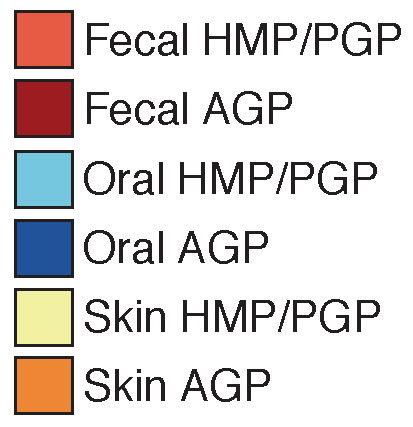
\includegraphics[width=0.20\textwidth]{pdfs-mod1/legend_agp_hmp_pgp.pdf}} &
\topalign{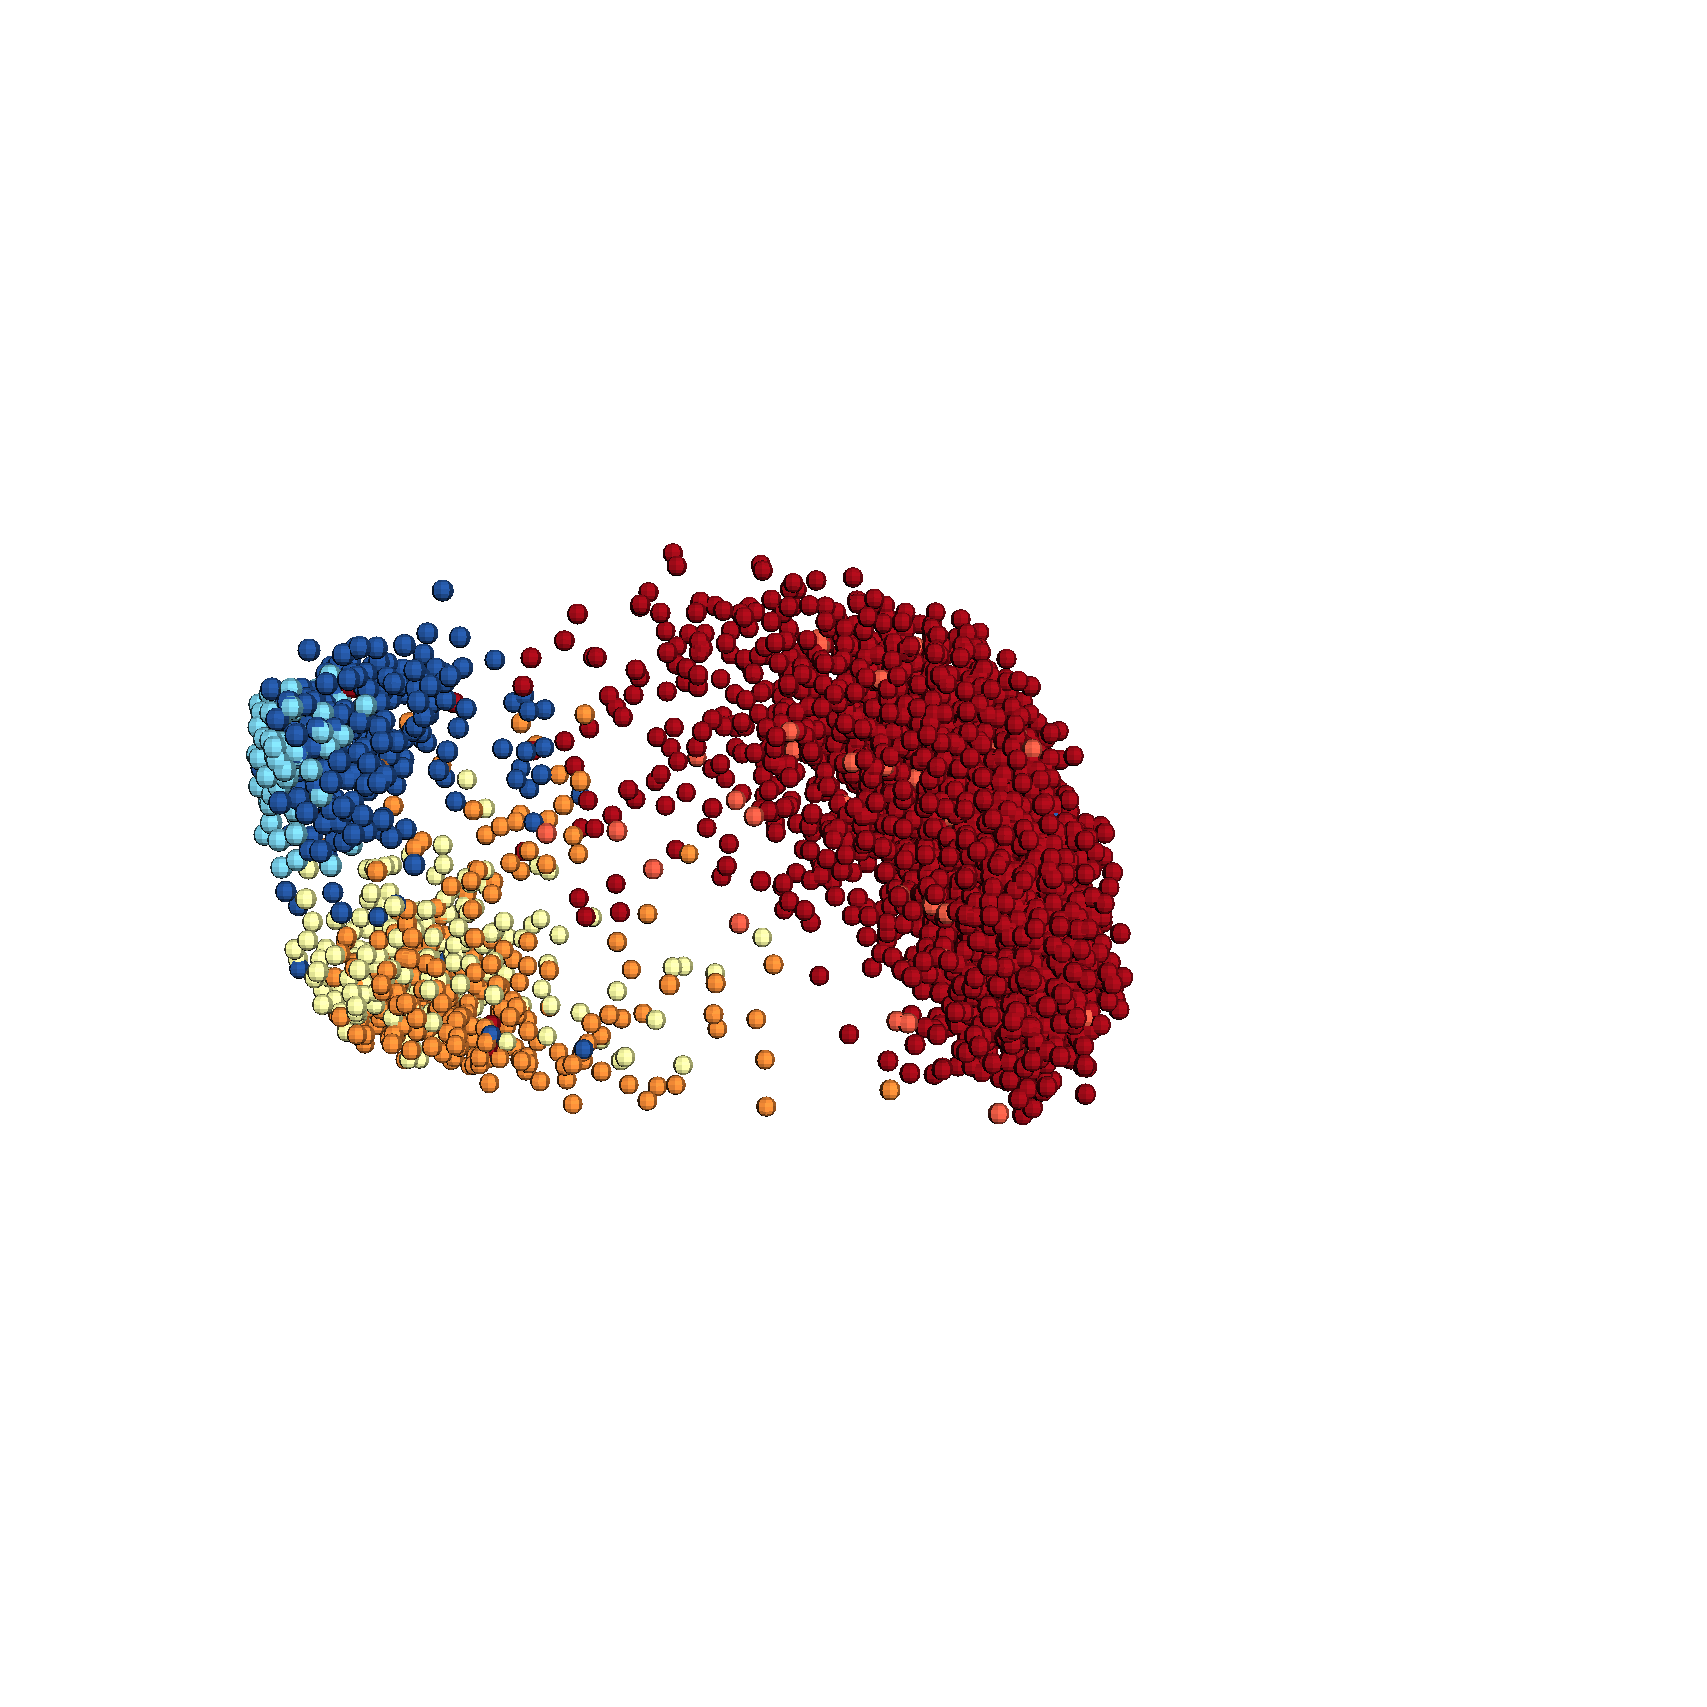
\includegraphics[trim=320 190 300 100, clip, width=0.39\textwidth]{pdfs-mod1/agp_pgp.pdf}}
\end{tabular}
}

\parbox{\textwidth}{
\captionof{figure}{Comparison of microbiota across studies and body sites. Each point represents the total microbiota in one individual at one body site. Points are colored by body site and project, showing that microbiota are distinct between the skin, the oral cavity, and the gut. Ovals show the approximate boundaries of each body site--study combination. {\bf (A)}~American Gut Project (AGP) and Human Microbiome Project (HMP). {\bf (B)}~AGP and Personal Genome Project (PGP). The results from AGP, HMP, and PGP show similar differences between body habitats.}
\vspace{-5mm}
}
\label{fig1} 
\end{framed}

% PAGE 2
\newpage

\parbox{4.5cm}{
	
\includegraphics[width=0.2\textwidth]{pdfs-mod1/logoshape.pdf}
}
\parbox{14cm}{
	\fontsize{20pt}{24pt}\selectfont
	Who is participating in the AGP?
}

% HEADING 2.1
\colorbox{agpMustard}{\parbox{\textwidth}{\vspace{1mm} \LARGE \centering Our participants \vspace{1mm}}}

We have sequenced \numSamples{} microbiota samples from \numParticipants{} people, including \pgpParticipants{} participants in the Personal Genome Project. We are just getting started, but already this number substantially exceeds the number of participants in other recent high-profile studies, including the Human Microbiome Project and the Global Gut study, which were published in the same issue of the scientific journal {\em Nature} last year.

% TABLE 1
\begin{framed}
\parbox{0.30\textwidth}{
\captionof{table}{Samples and participants in the American Gut project (AGP) compared to the Human Microbiome Project (HMP), Global Gut project (GG), and the Personal Genome Project microbiota component (PGP).}
}
\hspace{5mm}
\parbox{0.60\textwidth}{
{\footnotesize
\begin{tabular}{ l c c c c }													
\hline \addlinespace[1mm]													
 & HMP & GG	& PGP & AGP \\		
\hline \addlinespace[1mm]													
Subject Age & \hmpAge{} & \ggAge{} & \pgpAge{} & \agpAge{} \\
Subject Location & \hmpLocation{} & \ggLocation{} & \pgpLocation{} & \agpLocation{} \\
Total Samples & \hmpSamples{} & \ggSamples{} & \pgpSamples{} & \agpSamples{} \\
Total Participants & \hmpParticipants{} & \ggParticipants{} & \pgpParticipants{} & \agpParticipants{} \\
Sequences & \hmpSequences{} & \ggSequences{} & \pgpSequences{} & \agpSequences{} \\ \addlinespace[.5mm]
\hline															
\end{tabular}															
}
}
\vspace{-8mm}
{\fontsize{7pt}{7pt}\selectfont
\begin{my_itemize}
\item[] HMP -- The Human Microbiome Project Consortium, Structure, function and diversity of the healthy human microbiome. 2012. {\em Nature} 486: 202-214.
\item[] GG -- Global Gut, Yatsunenko et al. 2012. Human gut microbiome viewed across age and geography. {\em Nature} 486: 222-228.
\item[] PGP -- Personal Genome Project, participants and samples being continually added (unpublished data).
\item[] AGP -- American Gut Project, participants and samples being continually added.
\end{my_itemize}
\vspace{-3mm}
}
\label{tab1} 
\end{framed}

% FIGURE 2
\begin{framed}
\parbox{0.5\textwidth}{
\captionof{figure}{Comparison of gender, age and BMI across projects that characterize the human microbiota. Relative to the HMP, AGP contains more females, far more older and younger people, and a greater number of obese people. The concentration of older people is important because many health issues, including those that affect the gut, only appear later in life.}
}
\hspace{2mm}
\parbox{0.4\textwidth}{
\begin{tabular}{ c }
%{\hspace{1cm} \tenpt Gender \hspace{1.9cm} Age \hspace{1.4cm} BMI} \\ %\addlinespace[-2mm]
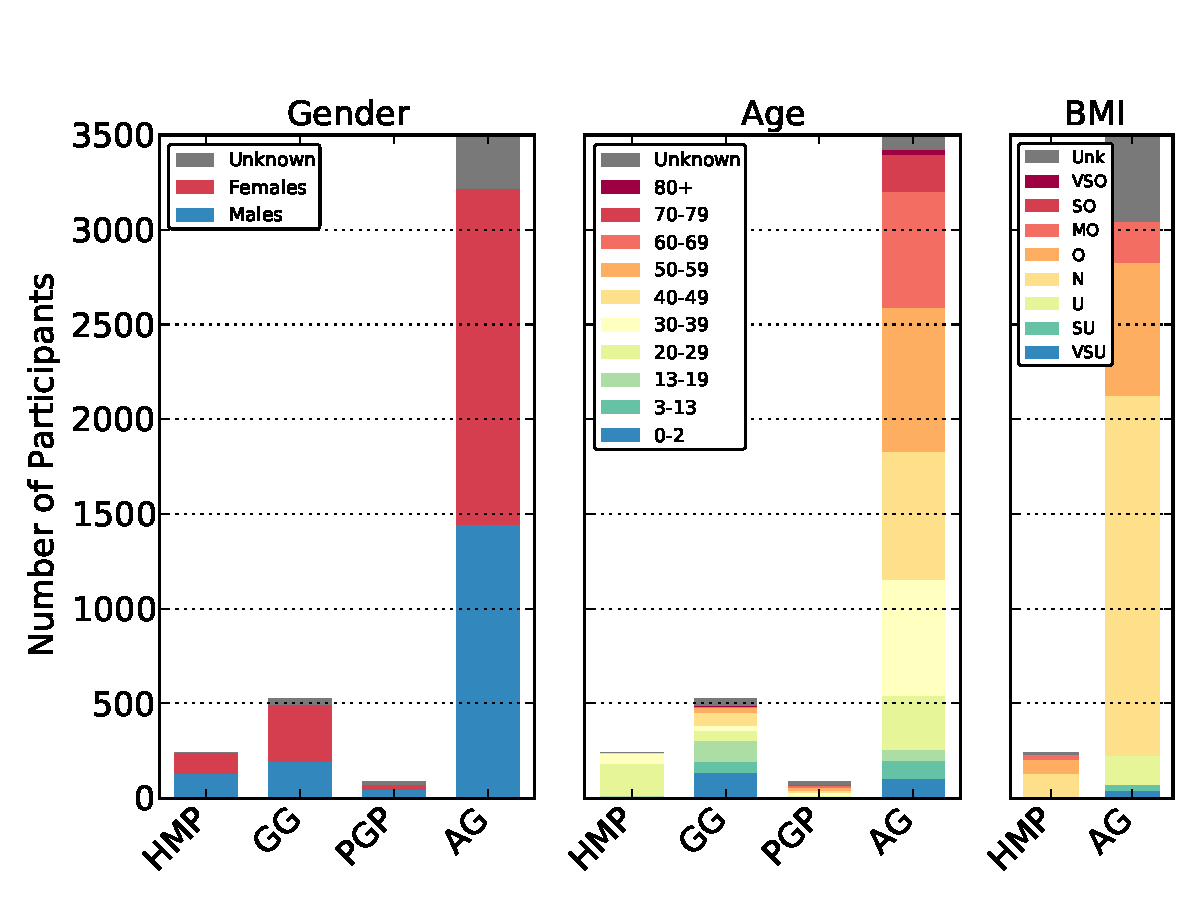
\includegraphics[trim=0 0 0 1.5cm, clip, scale=0.41]{pdfs-mod1/fig2.pdf}
\end{tabular}
}
\vspace{-4mm}
\label{fig2} 
\end{framed}

% FIGURE 3
\begin{framed}
\parbox{0.5\textwidth}{
\captionof{figure}{Diet and exercise regimes of the AGP population. According to self-reported data, the majority of our participants are omnivores who exercise frequently. Roughly half use vitamins regularly. As additional participants with more varied diet and exercise characteristics join the study (e.g., more vegans or more people who never exercise), we will be able to say more about how different lifestyles affect gut microbes and perhaps shed light on which lifestyle factors are associated with healthier gut bacteria.}
}
\hspace{2mm}
\parbox{0.4\textwidth}{
\begin{tabular}{ c }
%{\hspace{1.9cm} \tenpt Diet \hspace{0.9cm} Exercise frequency \hspace{0.05cm} Vitamins} \\ %\addlinespace[-2mm]
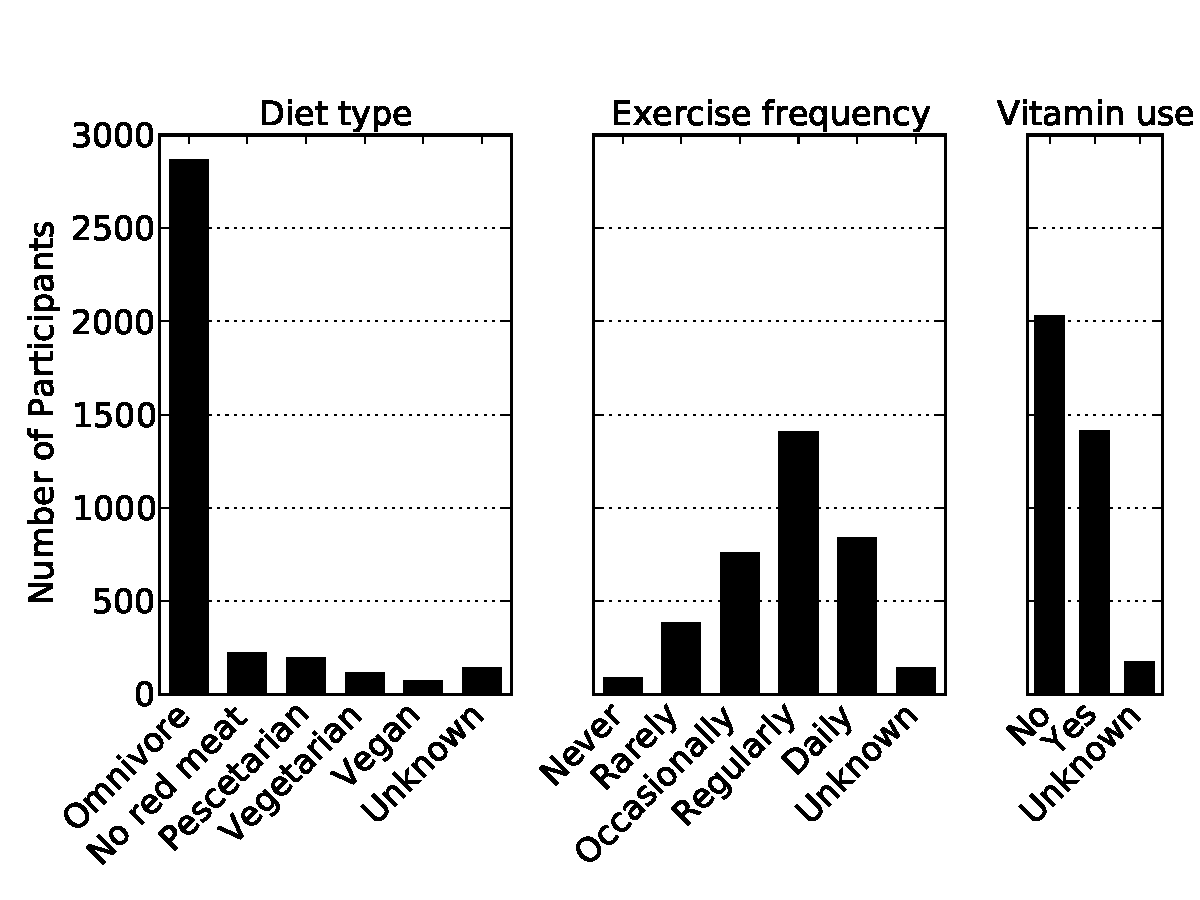
\includegraphics[trim=0 0 0 1.5cm, clip, scale=0.41]{pdfs-mod1/fig3.pdf}
\end{tabular}
}
\vspace{-4mm}
\label{fig3} 
\end{framed}

% PAGE 3
\newpage

\parbox{4.5cm}{
	
\includegraphics[width=0.2\textwidth]{pdfs-mod1/logoshape.pdf}
}
\parbox{14cm}{
	\fontsize{20pt}{24pt}\selectfont
	Who is living in your gut?
}

% HEADING 3.1
\colorbox{agpRust}{\parbox{\textwidth}{\vspace{1mm} \LARGE \centering \textcolor{white}{What kinds of microbes are in different sample types?} \vspace{1mm}}}

Just as seeing the major types of plants and animals (say, oaks versus pine trees) can give you a broad idea of what a traditional ecosystem looks like, knowing who is in your gut or mouth or skin provides a useful guide to what is going on in there.  Different parts of the body have very different microbes, as shown above in {\bf Figure 1}, but also at the same body site, different people have very different microbes. For example, some people have over 90\% Firmicutes in the gut, whereas other people have less than 1\%. Understanding the reasons for these differences is a major goal of the American Gut project.

The figures below show results at the level of bacterial phyla: a phylum is a big branch on the evolutionary tree of life. (For context, all arthropods, from shrimp to spiders, belong to a single phylum.) Many bacteria can be present in the gut, but not all are present in great numbers. For example, {\em E. coli} is  thought of as a classic gut bacterium because it is good at growing on a petri dish, not because it is a main component of the gut. At the phylum taxonomic level, the major players are Firmicutes and Bacteroidetes. Firmicutes include \emph{Clostridium} and \emph{Lactobacillus} species and many producers of the short-chain fatty acid butyrate. Bacteroidetes includes \emph{Bacteroides} and \emph{Prevotella}, both of which break down polysaccharides (big sugars).

% FIGURE 4 -- Y-AXIS ON FECAL PLOT ONLY, SHARED LEGEND?
\begin{framed}
\parbox{\textwidth}{
\begin{tabular}{ c c c @{} c }
{\eightpt ~~~~~Fecal} & {\eightpt ~~~~~Skin} & {\eightpt ~~~~~Oral} \\ \addlinespace[-4mm]
\topalign{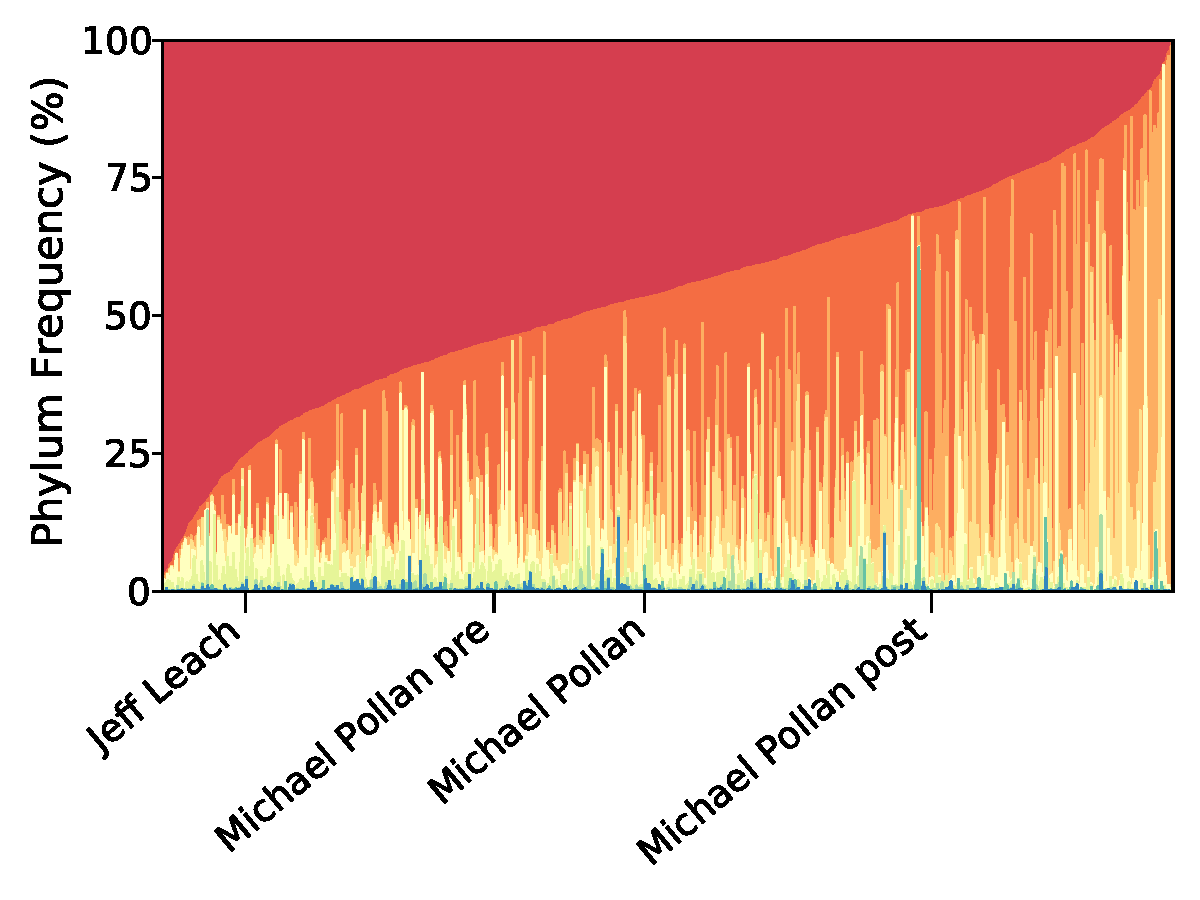
\includegraphics[width=0.25\textwidth]{pdfs-mod1/ag_plots_fecal_stack.pdf}} & \topalign{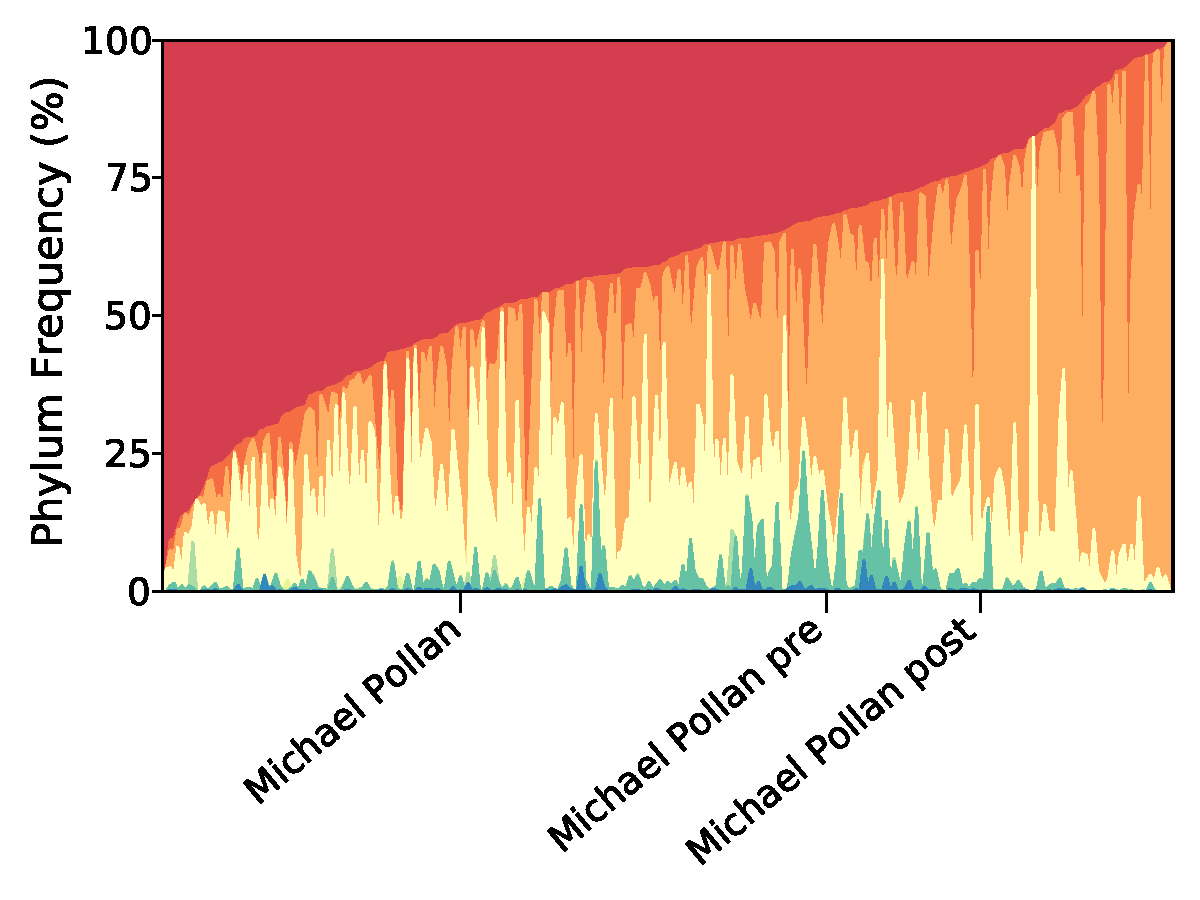
\includegraphics[width=0.25\textwidth]{pdfs-mod1/ag_plots_oral_stack.pdf}} & \topalign{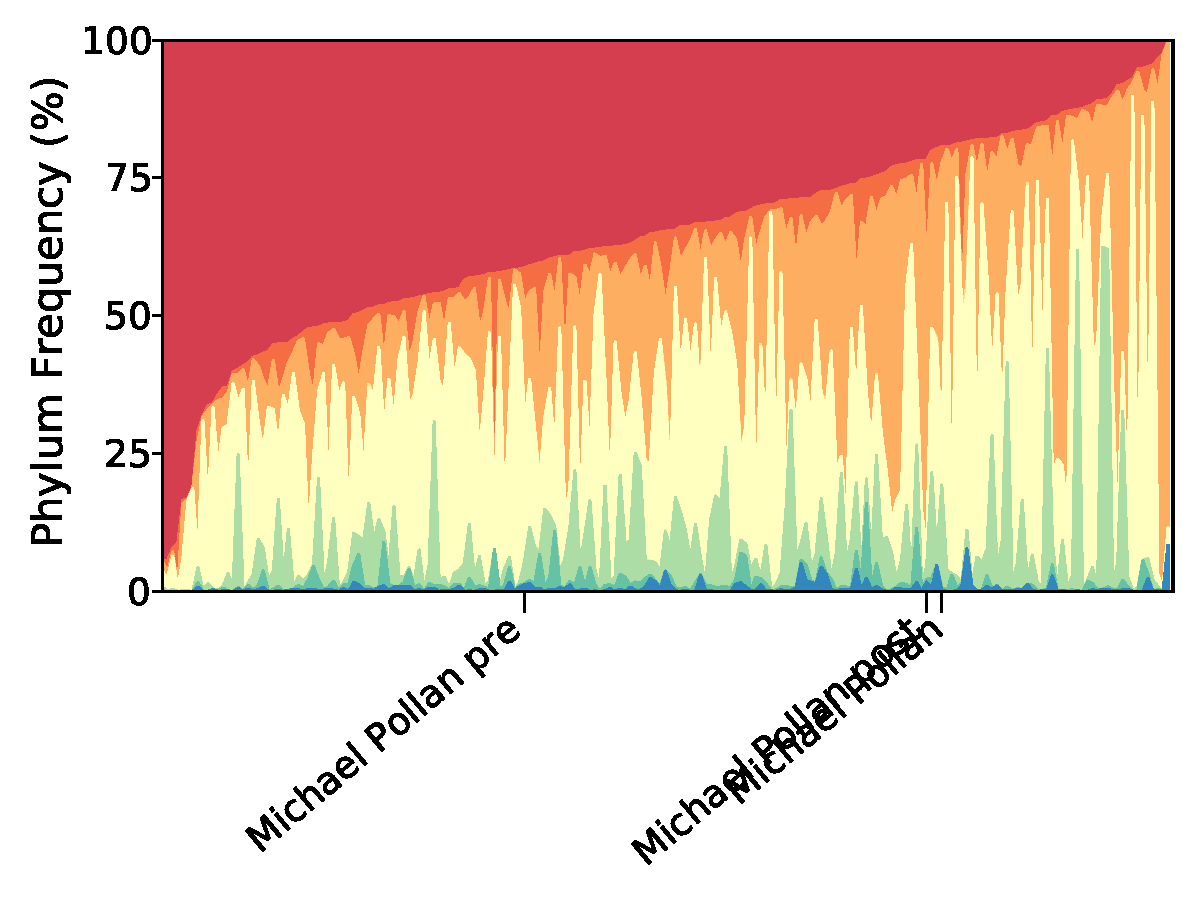
\includegraphics[width=0.25\textwidth]{pdfs-mod1/ag_plots_skin_stack.pdf}} & \topalign{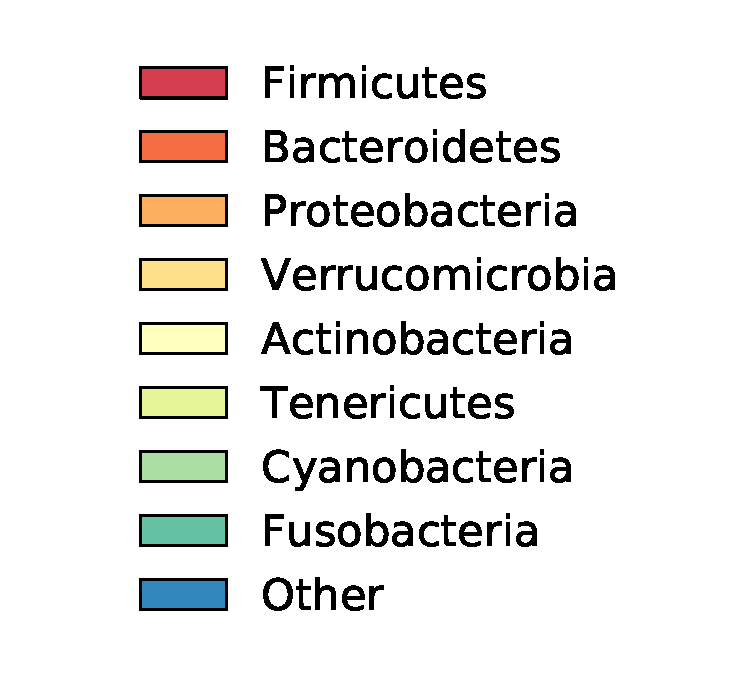
\includegraphics[width=0.23\textwidth]{pdfs-mod1/ag_plots_fecal_legend.pdf}} \end{tabular}
}
\parbox{\textwidth}{
\captionof{figure}{Microbial communities in fecal, oral and skin samples of AGP participants. Each color represents a different bacterial phylum, as shown in the legend. A few of our participants have agreed to have their samples identified for comparison. Jeff Leach is a paleo dieter; Michael Pollan is famously an omnivore (although his microbes changed post-antibiotics).} %Shannon Ford has celiac disease
\vspace{-5mm}
}
\label{fig4} 
\end{framed}

% HEADING 5.1
\colorbox{agpRust}{\parbox{\textwidth}{\vspace{1mm} \LARGE \centering \textcolor{white}{How much have we seen of the American Gut?} \vspace{1mm}}}

The gut is a complex ecosystem, far more like a rainforest than a desert.  Additionally, every person has a different mix of microbes in their gut.  Therefore, to truly understand how many kinds of microbes there are, we have to sample many people.  The AGP has sampled many more people than any other project, including the HMP. Therefore, for the types of people that participate in the AGP, we understand the range of kinds of microbes that exist. Now we just need to understand why and what factors affect them.

% FIGURE 5 -- NEED UPDATED PLOT
\begin{framed}
\parbox{0.45\textwidth}{
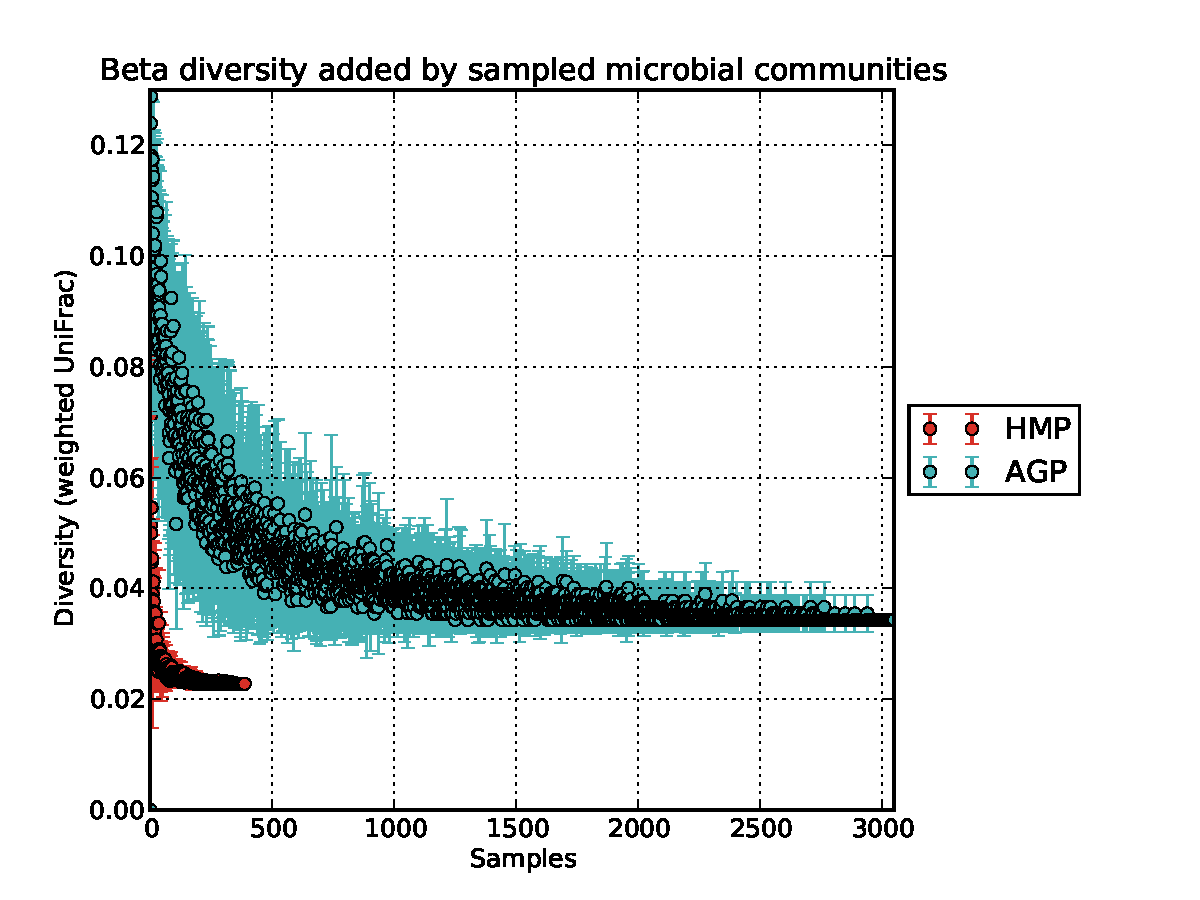
\includegraphics[width=0.4\textwidth]{pdfs-mod1/fig5.pdf}
}
\hspace{5mm}
\parbox{0.50\textwidth}{
\captionof{figure}{Diversity of the American Gut population relative to the population in the Human Microbiome Project. The x-axis shows the number of people characterized in the AGP or HMP; the y-axis shows how similar each additional sample is to the similar sample already in the dataset. Essentially, now that we have sampled more than \numParticipantsLowerEstimate{} people for every sample we add, we can find a similar sample that we already have data for. Adding more samples does not increase the number of new mixes of gut bacteria we see.}
}
\vspace{-2mm}
\label{fig5} 
\end{framed}
% PAGE 4
\newpage

\parbox{4.5cm}{
	
\includegraphics[width=0.2\textwidth]{pdfs-mod1/logoshape.pdf}
}
\parbox{14cm}{
	\fontsize{20pt}{24pt}\selectfont
	What affects your gut microbes?
}

% HEADING 4.1
\colorbox{agpBrown}{\parbox{\textwidth}{\vspace{1mm} \LARGE \centering \textcolor{white}{Factors that affect your gut habitat} \vspace{1mm}}}

As we saw in the last section, different people differ dramatically in what lives in their gut. Many factors, including antibiotic use, are known to change the composition of gut microbiota. But which of the many possible factors has the largest effect? Here we examine the effects of several factors that might affect your gut bacteria.

% FIGURE 6 -- NEED UPDATED PLOTS
\begin{framed}
\parbox{0.60\textwidth}{
\vspace{-3mm}
\begin{tabular}{ c }
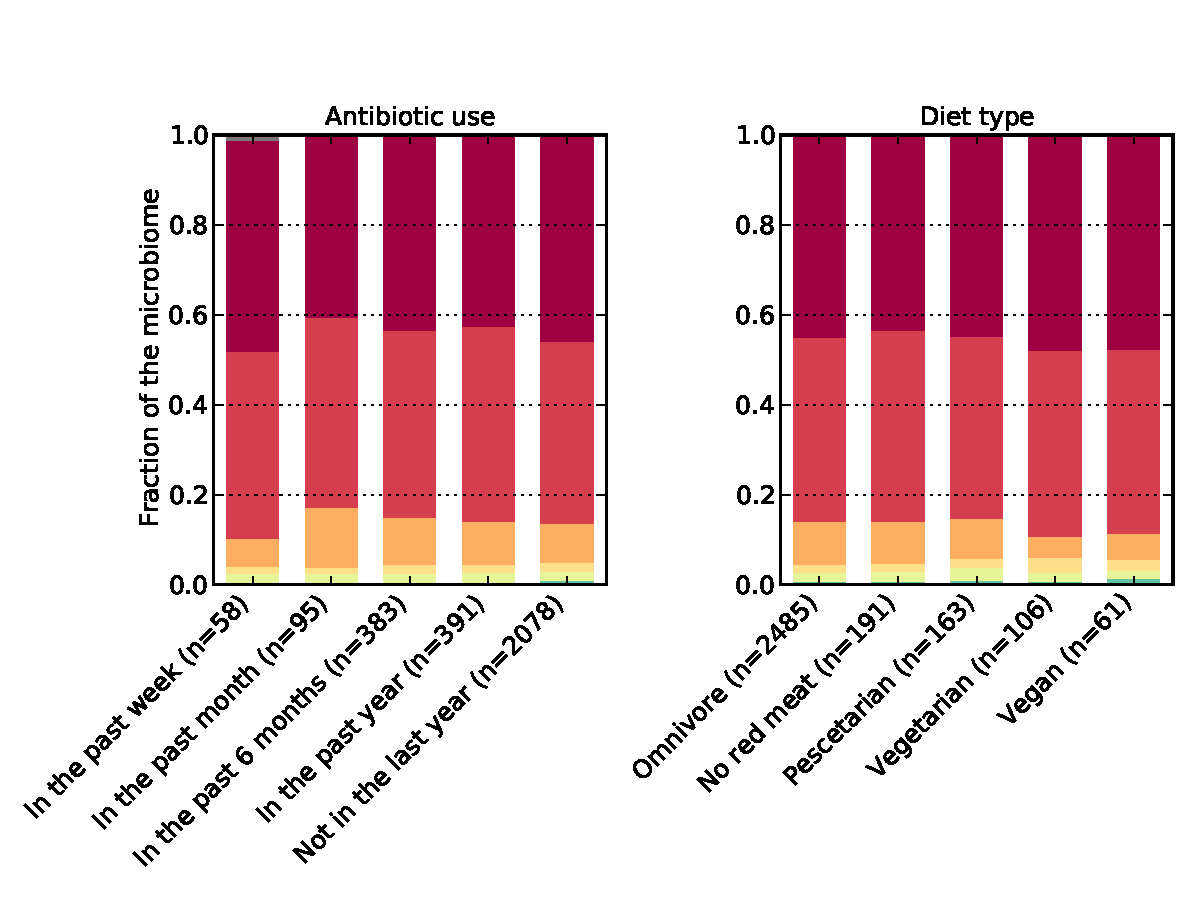
\includegraphics[trim=0 0 0 1.5cm, clip, width=0.6\textwidth]{pdfs-mod1/fig6_a.pdf} \\
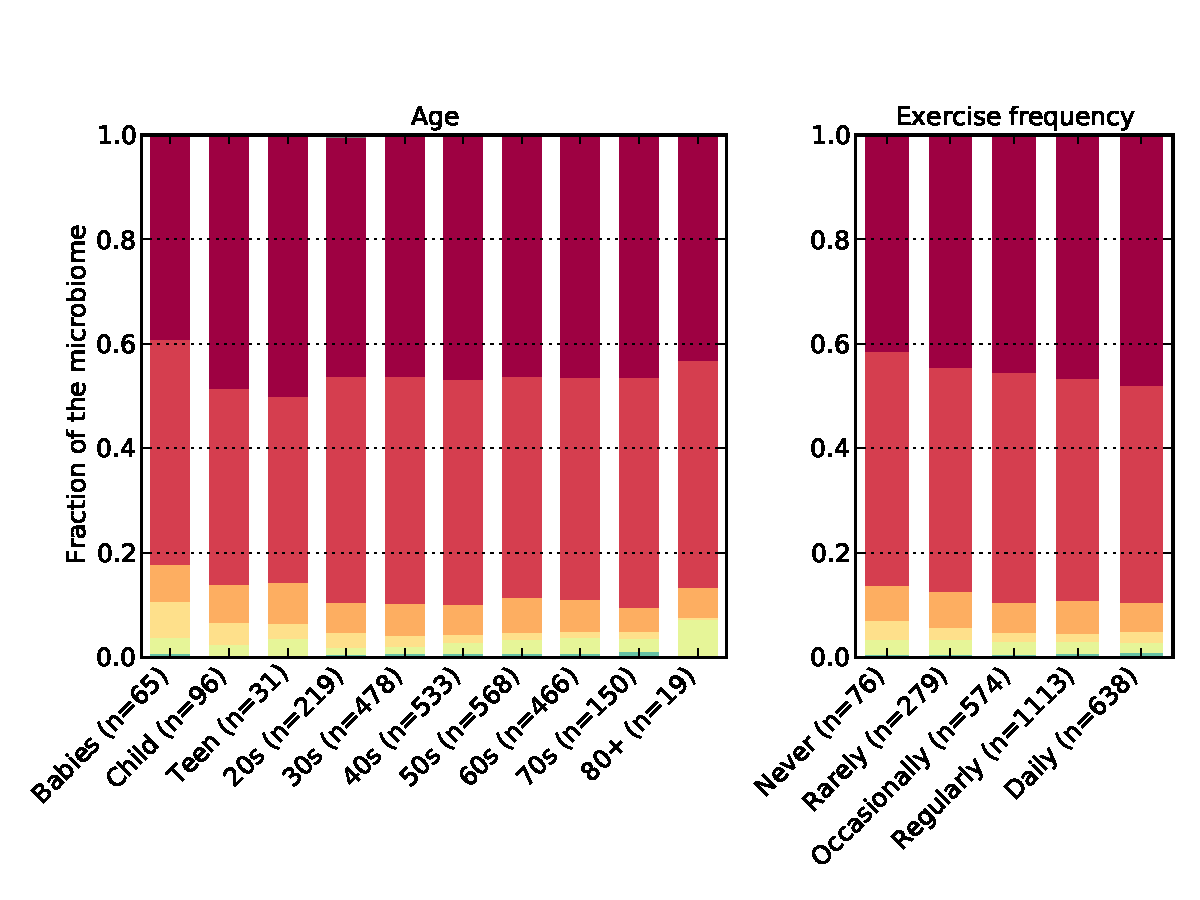
\includegraphics[trim=0 0 0 1.5cm, clip, width=0.6\textwidth]{pdfs-mod1/fig6_b.pdf}

\end{tabular}
}
\hspace{4mm}
\parbox{0.35\textwidth}{
\vspace{-3mm}
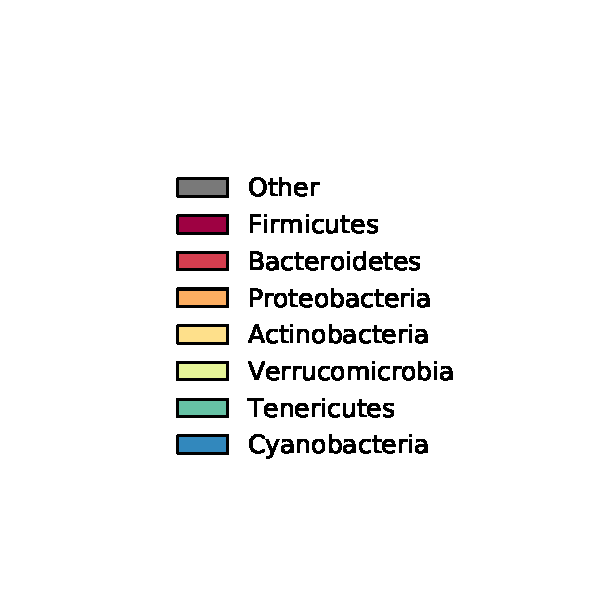
\includegraphics[trim=1cm 1cm 1cm 1cm, clip, width=0.30\textwidth]{pdfs-mod1/fig6_legend.pdf}
\captionof{figure}{Effects of diet, age, exercise frequency, and last antibiotic use on the average phylum-level variation in the gut bacteria of the American Gut participants. Average composition across many people is far less variable than the individual-level results shown in {\bf Figure~4}. This demonstrates that a lot of the variability we see is just differences between individuals and not the result of age or exercise or the other factors considered here. However, we do see some statistically significant differences: for example, younger people, especially babies, have more Proteobacteria (as expected from other published results), and vegetarians and vegans have fewer Proteobacteria (which technically means vegans are less like babies than are meat eaters; go figure). Antibiotic use within the past month or the past week also has a substantial effect at this level, although other research has shown that the results depend on which antibiotic it is and what was in that person's gut to begin with.}
\vspace{5mm}
}
\label{fig6} 
\end{framed}

% PAGE 5
\newpage

\parbox{4.5cm}{
	
\includegraphics[width=0.2\textwidth]{pdfs-mod1/logoshape.pdf}
}
\parbox{14cm}{
	\fontsize{20pt}{24pt}\selectfont
	What affects gut bacteria \\ in different studies?
}

% HEADING 5.1
\colorbox{agpBlue}{\parbox{\textwidth}{\vspace{1mm} \LARGE \centering \textcolor{white}{Where do you fit in?} \vspace{1mm}}}

By comparing our results to other studies that include participants from other parts of the world we can figure out where the American Gut and your gut fits into the global picture.  Although people from different countries tend to have different gut microbes (probably due to distinct diets), there are also factors, like age, that impact gut bacteria similarly, regardless of what country a person lives in.

% FIGURE 7 -- USE \fbox{\includegraphics[]{}} TO SHOW BOX AROUND FIGURE
\begin{framed}
\parbox{\textwidth}{
\begin{center}
\begin{tabular}{ l l @{} l }
\twelvept{\bf{A}} & & \\ \addlinespace[-4mm]
\topalign{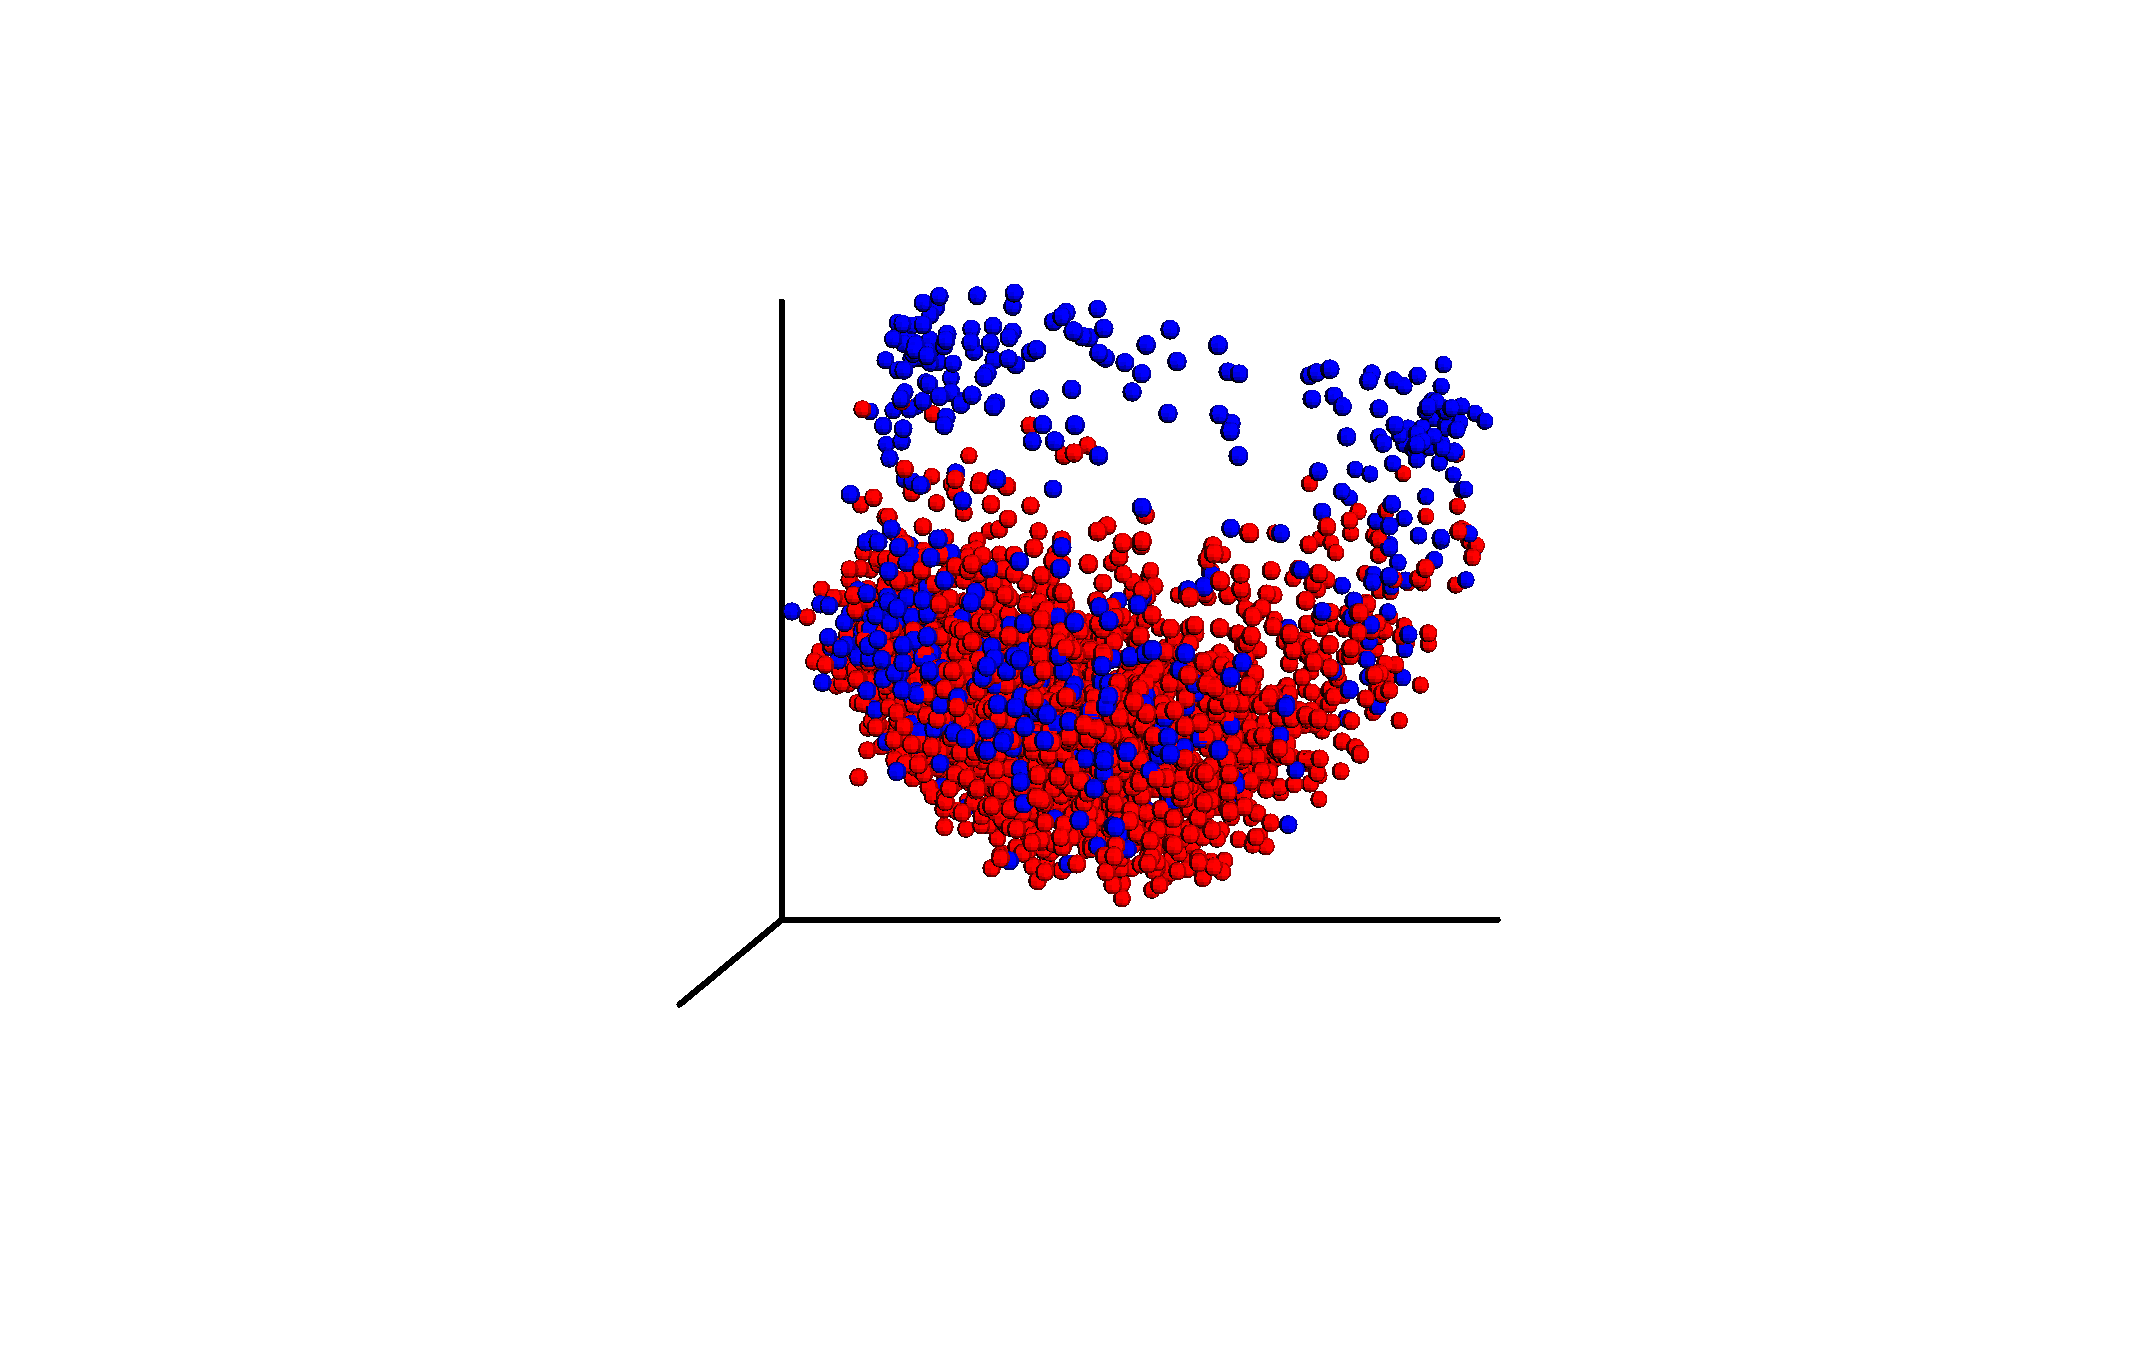
\includegraphics[trim=320 190 300 100, clip, width=0.39\textwidth]{pdfs-mod1/agp_gg_title.pdf}} &
\topalign{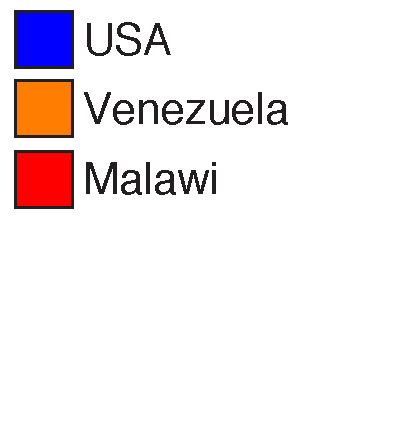
\includegraphics[width=0.20\textwidth]{pdfs-mod1/legend_agp_gg.pdf}} & \\ \addlinespace[4mm]
\twelvept{\bf{B}} & & \\ \addlinespace[-4mm]
\topalign{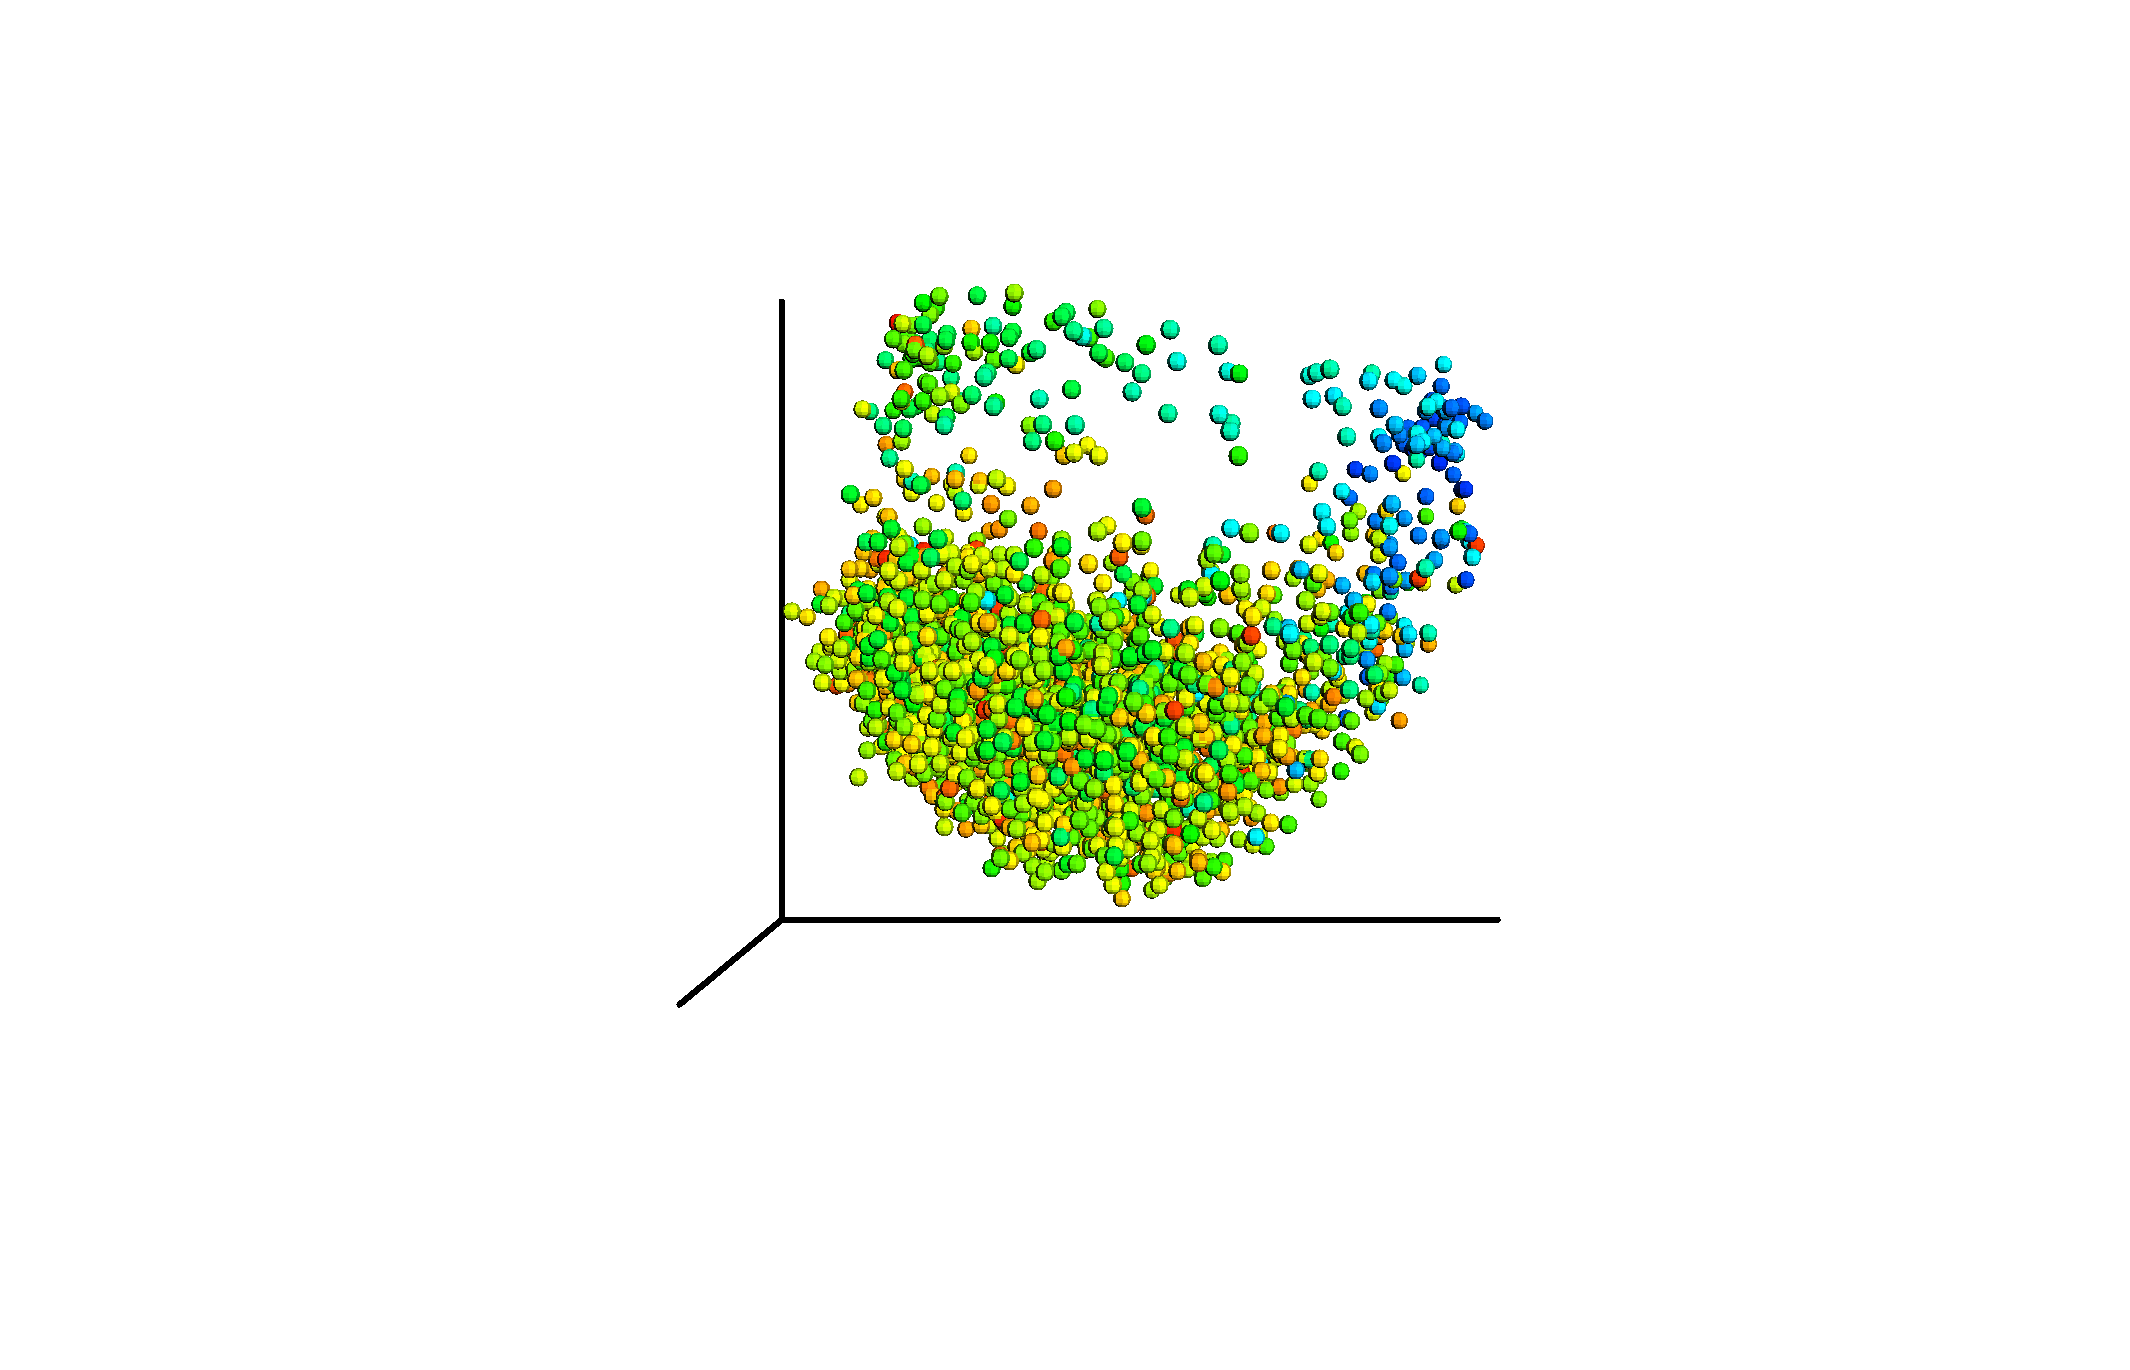
\includegraphics[trim=320 190 300 100, clip, width=0.39\textwidth]{pdfs-mod1/agp_gg_age.pdf}} &
\topalign{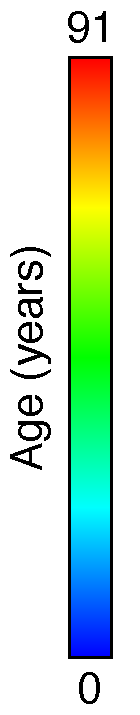
\includegraphics[width=0.07\textwidth]{pdfs-mod1/legend_age.pdf}} & 
\end{tabular}
\end{center}
}

\parbox{\textwidth}{
\captionof{figure}{This figure differentiates gut samples based on the country and age of subjects. {\bf (A)}~Western and non-Western guts are largely distinct, possibly owing to the higher consumption of processed sugars and carbohydrates in the Western diet. {\bf (B)}~Age has a large effect, with infants (in blue on the righthand side of the diagram) having very different gut microbiota from adults.}
\vspace{-5mm}
}
\label{fig7} 
\end{framed}

% PAGE 6
\newpage

\parbox{\textwidth}{
	\LARGE
	The American Gut Project would like to thank \ldots{}
}

\colorbox{agpGray}{\parbox{0.36\textwidth}{\vspace{1mm} \large \centering Contributors \vspace{1mm}}}
\hspace{1mm}
\colorbox{agpGray}{\parbox{0.623\textwidth}{\vspace{1mm} \large \centering Collaborators \vspace{1mm}}}

\parbox[t]{0.17\textwidth}{
\scriptsize{
Gail Ackermann\\
Katie Amato\\
Amnon Amir\\
Donna Berg--Lyons\\
Even Bolyen\\
Jeff DeReus\\
Justine Debelius\\
Rob Dunn\\
Merete Eggesbo\\
James Gaffney\\
Matt Gebert\\
Jack Gilbert\\
Grant Gogul\\
Antonio Gonzalez\\
Julia Goodrich\\
Steve Green\\
Kathy Holt\\
Greg Humphrey\\
Jim Huntley\\
Zehra Esra Ilhan\\
Jerry Kennedy\\
Rob Knight (co-founder)\\
Jeff Leach (co-founder)\\
Elijah Lovelace\\
Cathy Lozupone\\
Sebasti\'en Matamoros\\
Daniel Mayer\\
Kris Mayer\\
Daniel McDonald\\
}
}
\hspace{1mm}
\parbox[t]{0.17\textwidth}{
\scriptsize{
Jess Metcalf\\
Mike Minson\\
Jose Navas\\
Catherine Nicholas\\
Sarah Owens\\
Laura Parfrey\\
Juanma Peralta\\
Joe Petrosino\\
Meg Pirrung\\
Dorota Porazinska\\
Adam Robbins--Pianka\\
Jennifer Smilowitz\\
Se Jin Song\\
Emily TerAvest\\
Luke Thompson\\
Kumar Thurimella\\
Will Van Treuren\\
Luke Ursell\\
Yoshiki Vazquez--Baeza\\
Tim Vigers\\
Tony Walters\\
Sam Way\\
Sophie Weiss\\
Doug Wendel\\
Ulla Westermann\\
Dana Willner\\
Elaine Wolfe\\
Doug Woodhams\\
Zhenjiang Xu\\
}
} % JUST NAME AND INSTITUTION
\hspace{2mm}
\parbox[t]{0.623\textwidth}{
\scriptsize{
Martin J. Blaser, New York University\\
Jason Bobe, Harvard Medical School\\
Frederic Bushman, University of Pennsylvania\\
Patrice Cani, Universit\'e Catholique de Louvain\\
J. Gregory Caporaso, Northern Arizona University and Argonne National Labs\\
George Church, Harvard Medical School\\
Jose Clemente, Mount Sinai School of Medicine\\
Maria Gloria Dominguez, New York University and University of Puerto Rico Rio Pedras\\
Pieter Dorrestein, University of California, San Diego\\
Rob Dunn, North Carolina State University\\
Jonathan Eisen, University of California, Davis\\
Noah Fierer, University of Colorado, Boulder\\
J. Bruce German, University of California, Davis\\
Dirk Gevers, Broad Institute of MIT and Harvard\\
Jack Gilbert, University of Chicago and Argonne National Labs\\
Jessica Green, University of Oregon\\
Susan Holmes, Stanford University\\
Phil Hugenholtz, University of Queensland\\
Curtis Huttenhower, Harvard School of Public Health\\
Janet Jansson, Lawrence Berkeley National Laboratory\\
Rob Knight, University of Colorado, Boulder\\
Dan Knights, University of Minnesota\\
Rosa Krajmalnik-Brown, Arizona State University\\
Jeff Leach, Human Food Project\\
Carlito Lebrilla, University of California, Davis\\
Cecil M Lewis, University of Oklahoma\\
James Lewis, University of Pennsylvania\\
Ruth Ley, Cornell University\\
Catherine Lozupone, University of Colorado, Denver\\
David Mills, University of California, Davis\\
Joseph Petrosino, Baylor College of Medicine\\
Jeroen Raes, Flemish Institute of Biotechnology, Belgium\\
Jacques Ravel, University of Maryland School of Medicine\\
Jan Suchodolski, Texas A\&M University\\
Kelly Swanson, University of Illinois at Urbana-Champaign\\
Owen White, University of Maryland School of Medicine\\
Gary D. Wu, University of Pennsylvania\\
Ramnik Xavier, Massachusetts General Hospital
}
}

\begin{framed}
If you haven't joined American Gut please consider doing so -- we need your poo!  Join the 6,000+ other participants from around the world that have already donated to this unprecedented study to map the diversity of the American (Global) Gut.  Go to www.humanfoodproject.com/americangut/ and follow the links.  For more info email us at info@americangut.org.
\end{framed}

\colorbox{agpGray}{\parbox{0.66\textwidth}{\vspace{1mm} \large \centering Supporters \vspace{1mm}}}
\hspace{1mm}
\colorbox{agpGray}{\parbox{0.323\textwidth}{\vspace{1mm} \large \centering Sponsors \vspace{1mm}}}


\includegraphics[width=0.42\textwidth]{pdfs-mod1/s1.pdf}

\includegraphics[width=0.25\textwidth]{pdfs-mod1/s2.pdf}

\includegraphics[width=0.3\textwidth]{pdfs-mod1/s3.pdf}

\end{document}
